\documentclass[article]{jss}

%% -- LaTeX packages and custom commands ---------------------------------------

%% recommended packages
\usepackage{orcidlink,thumbpdf,lmodern}

\usepackage{amssymb}
\usepackage{amsmath}
\usepackage{siunitx}

%% another package (only for this demo article)
\usepackage{framed}

%% new custom commands
\newcommand{\class}[1]{`\code{#1}'}
\newcommand{\fct}[1]{\code{#1()}}


%% -- Article metainformation (author, title, ...) -----------------------------

%% - \author{} with primary affiliation (and optionally ORCID link)
%% - \Plainauthor{} without affiliations
%% - Separate authors by \And or \AND (in \author) or by comma (in \Plainauthor).
%% - \AND starts a new line, \And does not.
\author{Fernando Ferraz Ribeiro~\orcidlink{0000-0002-0685-4774}\\Universidade Federal da Bahia
   \And Gilney Figueira Zebende~\orcidlink{0000-0003-2420-9805}\\Universidade Estadual\\de Feira de Santana}
\Plainauthor{Fernando Ferraz Ribeiro, Gilney Figueira Zebende}
%  and $DMC_x^2$
%% - \title{} in title case
%% - \Plaintitle{} without LaTeX markup (if any)
%% - \Shorttitle{} with LaTeX markup (if any), used as running title
\title{A \proglang{Python}/\proglang{Zig} optimized and customizable implementation for the $\rho_{DCCA}$ and $DMC_x^2$ methods}
\Plaintitle{A Python/Zig optimized and customizable implementation for the Pdcca and DMCx2 methods}
\Shorttitle{\proglang{Python}/\proglang{Zig} implementation for the $\rho_{DCCA}$ and $DMC_x^2$}

%% - \Abstract{} almost as usual
\Abstract{
  This paper presents tha \pkg{Zebende}, a \proglang{Python} package written in \proglang{Python} and \proglang{Zig}, that calculates the $DFA$, $DCCA$ $\rho_{DCCA}$ and the $DMC_x^2$. The package presents an optimized algorithm that significantly improves the calculations speed. A comparison with other packages that calculates the .The package is also the first to implement the $DMC_x^2$ coefficient for any number of series.
}

%% - \Keywords{} with LaTeX markup, at least one required
%% - \Plainkeywords{} without LaTeX markup (if necessary)
%% - Should be comma-separated and in sentence case.
\Keywords{$\rho_{DCCA}$, $DMC_x^2$, optimization, \proglang{Python}, \proglang{Zig}}
\Plainkeywords{Pdcca, DMCx2, optimization, Python, Zig}

%% - \Address{} of at least one author
%% - May contain multiple affiliations for each author
%%   (in extra lines, separated by \emph{and}\\).
%% - May contain multiple authors for the same affiliation
%%   (in the same first line, separated by comma).
\Address{
  Fernando Ferraz Ribeiro\\
  Universidade Federal da Bahia\\
  Faculty of Achitecture\\
  Universit\"at Innsbruck\\
  Universit\"atsstr.~15\\
  6020 Innsbruck, Austria\\
  E-mail: \email{fernando.ribeiro@ufba.br}\\
  \emph{and}\\
  Centro Universitário Senai-Cimatec\\

  % URL: \url{https://www.zeileis.org/}
}

\begin{document}


%% -- Introduction -------------------------------------------------------------

%% - In principle "as usual".
%% - But should typically have some discussion of both _software_ and _methods_.
%% - Use \proglang{}, \pkg{}, and \code{} markup throughout the manuscript.
%% - If such markup is in (sub)section titles, a plain text version has to be
%%   added as well.
%% - All software mentioned should be properly \cite-d.
%% - All abbreviations should be introduced.
%% - Unless the expansions of abbreviations are proper names (like "Journal
%%   of Statistical Software" above) they should be in sentence case (like
%%   "generalized linear models" below).

\section{introduction} \label{sec:intro}

The $\rho_{DCCA}$~\citep{Zebende2011} is a widely used coefficient that measures the cross-correlation between tow non-stationary time series. It´s an extension of the Detrended Fluctuation Analysis ($DFA$)~\citep{Peng_1994} and the Detrended Cross-correlation Analysis ($DCCA$)~\citep{Podobnik2008}: while the $DFA$ calculates the self-affinity and long-memory properties of a time series data, and the $DCCA$ analyses power-law cross correlations between two different non-stationarity time series, the $\rho_{DCCA}$ coefficient quantifies this cross-correlation in simple values ranging from $-1$ to $1$, where $-1$ indicates a perfect anti-correlation between the series, $1$ a perfect correlation and zero ($0$) no correlation at all.

% rho DCCA applications

The Detrended Multiple Cross-Correlation Coefficient \citep{Zebende2018} ($DMC_x^2$) is a generalization of the $\rho_{DCCA}$ coefficient that correlates one time series (dependent variable) a number of time series (independent variables). The $DMC_x^2$ values ranges from zero ($0$), indicating no correlation to $1$, meaning perfect correlation or anti-correlation between the dependent and the independent variables.

% DMCx2 applications

This paper presents the \pkg{Zebende} \proglang{Python} package, an implementation of the $DFA$, $DCCA$, $\rho_{DCCCA}$, $DMC_x^2$ and utility functions related to the methods. In section \ref{sec:calculations} the steps for calculating the $\rho_{DCCCA}$ and $DMC_x^2$ are presented and discussed. Section \ref{sec:optimization} shows how this library was implemented, the optimization technics and the recommended steps to use the library. In Section \ref{sec:results} the \pkg{Zebende} package is compared with other packages for \proglang{Python} and \proglang{R} that calculates the $\rho_{DCCA}$ in terms of performance and usability, leading to the conclusions in \ref{sec:summary}.

\section{Algorithms of the coefficients}\label{sec:calculations}

The algorithms that calculates the $\rho_{DCCA}$ uses the $DFA$ and the $DCCA$ steps. The $DMC_x^2$ coefficient uses the $\rho_{DCCA}$ coefficient and, consequently, also embraces the $DFA$ and the $DCCA$. The $DFA$ method is described in six steps:


\begin{enumerate}\label{steps:dfa}

  \item Taking a time series \(\{x_{i}\}\) with \(i\) ranging from \(1\) to \(N\), the integrated series \(X_{k}\) is calculated by \(X_{k} = \sum_{i=1}^{k}\left[x_{i} - \langle x \rangle \right] \) with \(k\) also ranging from \(1\) to \(N\);
  \item the  \(X_{k}\) series is divided in \(N - n\) boxes of size \(n\)(time scale), each box containing \(n + 1\) values, starting in \(i\) up to \(i + n\);
  \item for each box, a polynomial (usually of degree 1) best fit is calculated, getting \(\widetilde{X}_{k, i}\) with \( i \le k \le (i + n) \) (detrended values);
  \item in each box is calculated: \(f_{DFA}^{2}(n, i) = \frac{1}{1+n} \sum_{k=i}^{i + n}(X_{k}-\widetilde{X}_{k, i})^{2}\)
  \item for all the boxes of a time scale, the $DFA$ is calculated as:\\[10pt]
        \(F_{DFA}(n) = \sqrt{\frac{1}{N - n} \sum_{i=1}^{N-n} f_{DFA}^{2}(n, i)}\);
  \item for a number of different timescales (n), with possible values \( 4 \le n \le \frac{N}{4}\) the \(F_{DFA}\) function is calculated to find a relation among \(F_{DFA} \times n\)

\end{enumerate}


The $DCCA$ method is very similar to the $DFA$ calculations. With the difference of analyzing two series while the $DFA$ evaluate properties of a single time series. It´s also a six steps process:


\begin{enumerate}
  \label{steps:DCCA}
  \item Taking two time series with the same length $\{x\alpha_{i}\}$ and \(\{x\beta_{i}\}\) with \(i\) ranging from \(1\) to \(N\),
        the integrated series \(X\alpha_{k}\) and \(X\beta_{k}\) are calculated by
        \(X_{k} = \sum_{i=1}^{k}\left[x_{i} - \langle x \rangle \right] \) for each series, with \(k\) also ranging from \(1\) to \(N\);
  \item \(X\alpha_{k}\) and \(X\beta_{k}\) series are divided in \(N - n\) boxes of size \(n\)(time scale), each box containing \(n + 1\) values, starting in \(i\) up to \(i + n\);
  \item for each box, a polynomial (usually of degree 1) best fit is calculated, getting
        $\widetilde{X\alpha}_{k, i}$ and $\widetilde{X\beta}_{k, i}$,
        for series $\{x\alpha_{i}\}$ and $\{x\beta_{i}\}$ respectively,
        with \( i \le k \le (i + n) \) (detrended values);
  \item in each box is calculated: $f_{DCCA}^{2}(n, i) =
        \frac{1}{1+n} \sum_{k=i}^{i + n}(X\alpha_{k}-\widetilde{X\alpha}_{k, i}) \times (X\beta_{k}-\widetilde{X\beta}_{k, i})$
  \item for all the boxes of a time scale, the $DCCA$ is calculated as:\\[10pt]
        $F_{DCCA}^{2}(n) =\frac{1}{N - n} \sum_{i=1}^{N-n} f_{DCCA}^{2}(n, i)$;
  \item for a number of different timescales (n), with possible values
        $4 \le n \le \frac{N}{4}$ the $F_{DCCA}^{2}$ function is calculated to find a relation among
        $F_{DCCA}^{2} \times n$
\end{enumerate}
 
Comparing the algorithms, the first three are basically identical, the only difference is that the $DCCA$ method apply those steps to two series. The step four of the $DFA$ is essentially an application of the variance calculation and the equivalent step of the $DCCA$ is a covariance between the two series. Step five calculates the square root of the mean of the variances calculated in  in each box for the $DFA$, in the $DCCA$, the mean of the covariances calculated for each box is calculated in stead. The last step,in both cases, is more a reminder to repeat the respective previous operations for a number of difference time scales.

The $\rho_{DCCA}$ is measured using Eq. \ref{eq:p_dcca}. Considering the relation between $DFA$ and variance and $DCCA$ and covariance, the $\rho_{DCCA}$ resembles Pearson correlation for a time scale $n$.

\begin{equation}
  {\rho}_{DCCA}(n) = \frac{F_{DCCA~(x\alpha,~x\beta)}^{2}(n)}
  {F_{DFA~(x\alpha)}(n) \times F_{DFA~(x\beta)}(n)}
  \label{eq:p_dcca}
\end{equation}

The $DMC_x^2$ is a generalization of the $\rho_{DCCA}$ that calculates the correlation between one time-series $\left\lbrace Y \right\rbrace $, as the  dependent variable, and a number $j$ of time-series $\left\lbrace X_{1} \right\rbrace $, $\left\lbrace X_{2} \right\rbrace $, $\left\lbrace X_{3} \right\rbrace $, $\dots $, $\left\lbrace X_{j} \right\rbrace $ defined as independent variables. The coefficient is expressed mathematically as:

\begin{equation}
  {DMC}_{x}^{2}  \equiv \rho_{Y,X_{i}}(n)^{T} \times \rho^{-1}(n) \times \rho_{Y,X_{i}}(n)
  \label{eq:dmcx2}
\end{equation}

In Eq. \ref{eq:dmcx2}, $\rho^{-1}(n)$ represent the inverse of a matrix populated by all possible combinations of $\rho_{DCCA}$ between independent variables. In Eq. \ref{eq:p_dcca_matrix}, value $\rho_{X_{1},X_{2}}(n)$, for instance, is the $\rho_{DCCA}$ for independent variables $X_{1}$ and $X_{2}$ calculated with time scale $n$, occupying position $\rho_{1 2}$ of the matrix. Two fundamental characteristics: the first is that the main diagonal values are all ones, since it's position in the matrix denotes the calculation of a correlation between a series and itself. Second, the matrix is symmetric in relation to the main diagonal, as the $\rho_{DCCA}$ is evaluated a commutative expression. 

\begin{equation}
  \rho^{-1}(n) = \left(\begin{matrix}
    1                     & \rho_{X_{1},X_{2}}(n) & \rho_{X_{1},X_{3}}(n) & \dots & \rho_{X_{1},X_{j}}(n) \\
    \rho_{X_{2},X_{1}}(n) & 1                     & \rho_{X_{2},X_{3}}(n) & \dots & \rho_{X_{2},X_{j}}(n) \\
    \vdots                & \vdots                & \vdots                & \dots & \vdots                \\
    \rho_{X_{j},X_{1}}(n) & \rho_{X_{j},X_{2}}(n) & \rho_{X_{j},X_{3}}(n) & \dots & 1                     \\
  \end{matrix}\right)^{-1}
  \label{eq:p_dcca_matrix}
\end{equation}

At last Eq. \ref{eq:rhocol} represent the transposed vector of the $\rho_{Y,X_{i}}(n)$ between the depended variable $\left\lbrace Y \right\rbrace $ and each $\left\lbrace X_{i} \right\rbrace $ independent variable for a given time scale $n$. 

\begin{equation} \label{eq:rhocol}
  \rho_{Y,X_i}(n)^T=[\rho_{Y,X_1}(n), \rho_{Y,X_2}(n),\cdots,\rho_{Y,X_j}(n)]
\end{equation}

The $\rho_{DCCA}$ and the $DMC_x^2$ should be evaluated in a number of time scales ($n$) to analyze the characteristics of each coefficient.

%% -- Manuscript ---------------------------------------------------------------

%% - In principle "as usual" again.
%% - When using equations (e.g., {equation}, {eqnarray}, {align}, etc.
%%   avoid empty lines before and after the equation (which would signal a new
%%   paragraph.
%% - When describing longer chunks of code that are _not_ meant for execution
%%   (e.g., a function synopsis or list of arguments), the environment {Code}
%%   is recommended. Alternatively, a plain {verbatim} can also be used.
%%   (For executed code see the next section.)

\section{Zebende package: implementation and optimization} \label{sec:optimization}


\begin{figure}[t!]
  \centering
  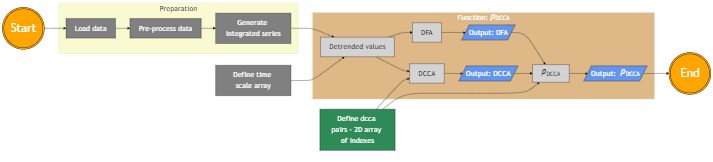
\includegraphics{./figs/pdcca_cart.png}
  \caption{\label{fig:pdcca_flow}Flowchart for the $\rho_{DCCA}$ package usage}
  \end{figure}


  \begin{figure}[t!]
    \centering
    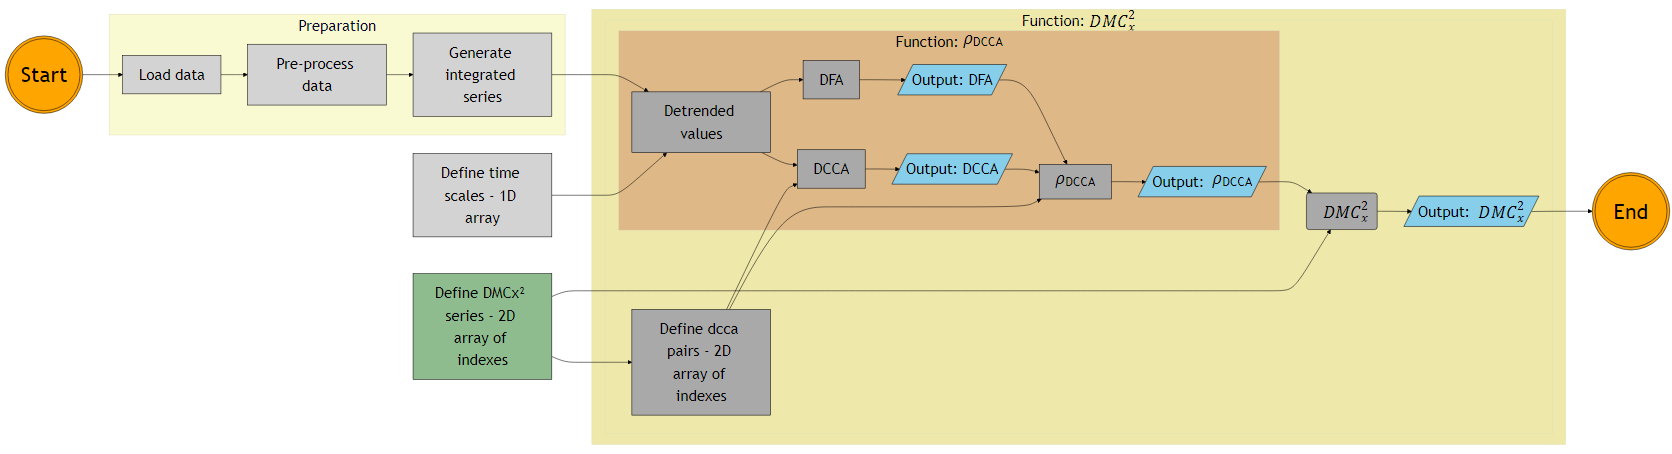
\includegraphics{./figs/dmc_chart.png}
    \caption{\label{fig:pdcca_flow}Flowchart for the $DMC_x^2$ package usage}
    \end{figure}
  


%% -- Illustrations ------------------------------------------------------------

%% - Virtually all JSS manuscripts list source code along with the generated
%%   output. The style files provide dedicated environments for this.
%% - In R, the environments {Sinput} and {Soutput} - as produced by Sweave() or
%%   or knitr using the render_sweave() hook - are used (without the need to
%%   load Sweave.sty).
%% - Equivalently, {CodeInput} and {CodeOutput} can be used.
%% - The code input should use "the usual" command prompt in the respective
%%   software system.
%% - For R code, the prompt "R> " should be used with "+  " as the
%%   continuation prompt.
%% - Comments within the code chunks should be avoided - these should be made
%%   within the regular LaTeX text.

\section{Results} \label{sec:results}




%% -- Summary/conclusions/discussion -------------------------------------------

\section{Summary and discussion} \label{sec:summary}


%% -- Optional special unnumbered sections -------------------------------------

% \section*{Computational details}

% \begin{leftbar}
%   If necessary or useful, information about certain computational details
%   such as version numbers, operating systems, or compilers could be included
%   in an unnumbered section. Also, auxiliary packages (say, for visualizations,
%   maps, tables, \dots) that are not cited in the main text can be credited here.
% \end{leftbar}

% The results in this paper were obtained using
% \proglang{R}~3.4.1 with the
% \pkg{MASS}~7.3.47 package. \proglang{R} itself
% and all packages used are available from the Comprehensive
% \proglang{R} Archive Network (CRAN) at
% \url{https://CRAN.R-project.org/}.


% \section*{Acknowledgments}

% \begin{leftbar}
%   All acknowledgments (note the AE spelling) should be collected in this
%   unnumbered section before the references. It may contain the usual information
%   about funding and feedback from colleagues/reviewers/etc. Furthermore,
%   information such as relative contributions of the authors may be added here
%   (if any).
% \end{leftbar}


%% -- Bibliography -------------------------------------------------------------
%% - References need to be provided in a .bib BibTeX database.
%% - All references should be made with \cite, \citet, \citep, \citealp etc.
%%   (and never hard-coded). See the FAQ for details.
%% - JSS-specific markup (\proglang, \pkg, \code) should be used in the .bib.
%% - Titles in the .bib should be in title case.
%% - DOIs should be included where available.

\bibliography{refs}


%% -- Appendix (if any) --------------------------------------------------------
%% - After the bibliography with page break.
%% - With proper section titles and _not_ just "Appendix".

% \newpage

% \begin{appendix}

%   \section{More technical details} \label{app:technical}

%   \begin{leftbar}
%     Appendices can be included after the bibliography (with a page break). Each
%     section within the appendix should have a proper section title (rather than
%     just \emph{Appendix}).

%     For more technical style details, please check out JSS's style FAQ at
%     \url{https://www.jstatsoft.org/pages/view/style#frequently-asked-questions}
%     which includes the following topics:
%     \begin{itemize}
%       \item Title vs.\ sentence case.
%       \item Graphics formatting.
%       \item Naming conventions.
%       \item Turning JSS manuscripts into \proglang{R} package vignettes.
%       \item Trouble shooting.
%       \item Many other potentially helpful details\dots
%     \end{itemize}
%   \end{leftbar}


%   \section[Using BibTeX]{Using \textsc{Bib}{\TeX}} \label{app:bibtex}

%   \begin{leftbar}
%     References need to be provided in a \textsc{Bib}{\TeX} file (\code{.bib}). All
%     references should be made with \verb|\cite|, \verb|\citet|, \verb|\citep|,
%     \verb|\citealp| etc.\ (and never hard-coded). This commands yield different
%     formats of author-year citations and allow to include additional details (e.g.,
%     pages, chapters, \dots) in brackets. In case you are not familiar with these
%     commands see the JSS style FAQ for details.

%     Cleaning up \textsc{Bib}{\TeX} files is a somewhat tedious task -- especially
%     when acquiring the entries automatically from mixed online sources. However,
%     it is important that informations are complete and presented in a consistent
%     style to avoid confusions. JSS requires the following format.
%     \begin{itemize}
%       \item JSS-specific markup (\verb|\proglang|, \verb|\pkg|, \verb|\code|) should
%             be used in the references.
%       \item Titles should be in title case.
%       \item Journal titles should not be abbreviated and in title case.
%       \item DOIs should be included where available.
%       \item Software should be properly cited as well. For \proglang{R} packages
%             \code{citation("pkgname")} typically provides a good starting point.
%     \end{itemize}
%   \end{leftbar}

% \end{appendix}

%% -----------------------------------------------------------------------------


\end{document}
